\section{Deterministické konečné automaty}\label{sec:det-automaty}

Již jsme si představili jazyky jakožto prostředek pro reprezentaci vstupů pro konečné automaty. Stále jsme si ovšem neřekli, co to ten automat vlastně je. Podobně jako v definici grafu, kdy máme uspořádanou dvojici vrcholů a hran, i zde bude myšlenka velice podobná.
\begin{definition}[Deterministický končný automat]
    \emph{Deterministický konečný automat} je uspořádaná pětice $A=(Q,\Sigma,\delta,q_0,F)$, kde
    \begin{itemize}
        \item $Q$ je konečná \emph{množina stavů},
        \item $\Sigma$ je abeceda, z níž sestávají slova na vstupu,
        \item $\delta$ je tzv. \emph{přechodová funkce} $Q\times\Sigma\rightarrow Q$ udávající přechody mezi stavy,
        \item $q_0\in Q$ je \emph{počáteční stav} automatu
        \item a $F\subseteq Q$ je \emph{množina přijímajících stavů}.
    \end{itemize}
\end{definition}
Automaty zakreslujeme pomocí stavového diagramu (formálně orientovaného grafu), přičemž
\begin{itemize}
    \item \emph{vrcholy} jsou jednotlivé stavy automatu (dvojitý kruh značí přijímající stav a do počátečního stavu vede šipka ``odnikud'')
    \item a \emph{šipky} reprezentují přechody mezi stavy.
\end{itemize}
Na začátku výpočtu dostane automat na vstupu slovo $w\in\Sigma^*$, které čte znak po znaku (zleva doprava). Začínáme v počátečním stavu $q_0$, přičemž vždy podle následujícího čteného znaku se automat přesouvá do nového stavu. Přechodová funkce $\delta:Q\times\Sigma\rightarrow Q$ nám udává pro každou dvojici $(q,a)$, kde $q$ je stav, v němž se automat nachází a $a$ je aktuálně čtený znak, do jakého stavu se má automat přesunout. Pokud na konci čtení slova $w$ skončí výpočet v jednom z přijímajících stavů, pak automat slovo přijímá. V opačném případě, kdy výpočet neskončí v přijímajícím stavu nebo přechod pro určitý znak z určitéhoi stavu není definovaný, pak výpočet končí a automat slovo nepřijímá.
\begin{example}
    Máme automat $A=(Q,\Sigma,\delta,q_0,F)$, kde
    \begin{itemize}
        \item $Q=\set{q_0,q_1,q_2}$,
        \item $q_0$ je počáteční stav,
        \item $F=\set{q_2}$,
        \item $\Sigma=\set{0,1}$,
        \item Přechodová funkce $\delta$ (viz tabulka \ref{tab:prechodova-funkce-A}):
        \begin{itemize}
            \item $\delta(q_0,0)=q_1$,
            \item $\delta(q_0,1)=q_2$,
            \item $\delta(q_0,0)=q_2$,
            \item $\delta(q_0,1)=q_2$.
        \end{itemize}
    \end{itemize}
    Schéma automatu lze vidět na obrázku \ref{fig:automat-A} níže.
    \begin{figure}[h]
        \centering
        \centering
        \begin{center}
            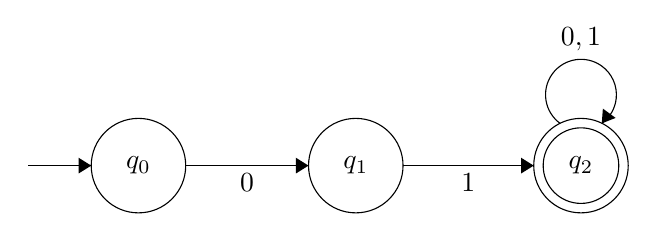
\begin{tikzpicture}[scale=0.2]
            \tikzstyle{every node}+=[inner sep=0pt]
            \draw [black] (18.8,-30.5) circle (3);
            \draw (18.8,-30.5) node {$q_0$};
            \draw [black] (32.6,-30.5) circle (3);
            \draw (32.6,-30.5) node {$q_1$};
            \draw [black] (46.9,-30.5) circle (3);
            \draw (46.9,-30.5) node {$q_2$};
            \draw [black] (46.9,-30.5) circle (2.4);
            \draw [black] (21.8,-30.5) -- (29.6,-30.5);
            \fill [black] (29.6,-30.5) -- (28.8,-30) -- (28.8,-31);
            \draw (25.7,-31) node [below] {$0$};
            \draw [black] (35.6,-30.5) -- (43.9,-30.5);
            \fill [black] (43.9,-30.5) -- (43.1,-30) -- (43.1,-31);
            \draw (39.75,-31) node [below] {$1$};
            \draw [black] (45.577,-27.82) arc (234:-54:2.25);
            \draw (46.9,-23.25) node [above] {$0,1$};
            \fill [black] (48.22,-27.82) -- (49.1,-27.47) -- (48.29,-26.88);
            \draw [black] (11.8,-30.5) -- (15.8,-30.5);
            \fill [black] (15.8,-30.5) -- (15,-30) -- (15,-31);
            \end{tikzpicture}
        \end{center}
        \caption{Schéma automatu $A$ a tabulka přechodové funkce $\delta$}
        \label{fig:automat-A}
    \end{figure}
    \begin{table}[h]
        \centering
        \begin{tabular}{c|cc}
        & $0$           & $1$           \\ \hline
        $q_0$      & $q_1$        & -- \\
        $q_1$      & -- & $q_2$        \\
        $q_2$      & $q_2$        & $q_2$        \\
        \end{tabular}
        \caption{Tabulka přechodové funkce $\delta$ automatu $A$}
        \label{tab:prechodova-funkce-A}
    \end{table}
\end{example}